
%\begin{equation}
%		nh = \oint p \, dq = 
%	\end{equation}
%	$E/F < L$ esete:
%	\begin{equation}
%		2\int_0^{E/F}\sqrt{2m\left( E-Fx \right)}\,dx = -\frac{2}{3mF}\left(2m\left( E-Fx \right)\right)^{\frac{3}{2}}\bigg \rvert_0^{E/F} = \frac{4\sqrt{2m}E^{3/2}}{3F}
%	\end{equation}
%	\begin{equation}
%		E_n = \left(\frac{3nhF}{4\sqrt{2m}}\right)^{2/3}
%	\end{equation}
%	$E/F > L$ esete:
%	\begin{equation}
%		-\frac{2}{3mF}\left(2m\left( E-Fx \right)\right)^{\frac{3}{2}}\bigg \rvert_0^{L} = \frac{4\sqrt{2m}}{3F}\left(E^{3/2} - \left(E - FL\right)^{3/2}\right) = nh
%	\end{equation}
%	$E \gg FL$ esetén a különbség az $E^{3/2}$ függvény deriváltjának segítségével helyettesíthető:
%	\begin{equation}
%		nh \approx 2\sqrt{2m}E^{1/2}L
%	\end{equation}
%	\begin{equation}
%		E_n \approx \frac{n^2h^2}{8mL^2}
%	\end{equation}
%	
%	\begin{figure}[H]
%		\centering
%		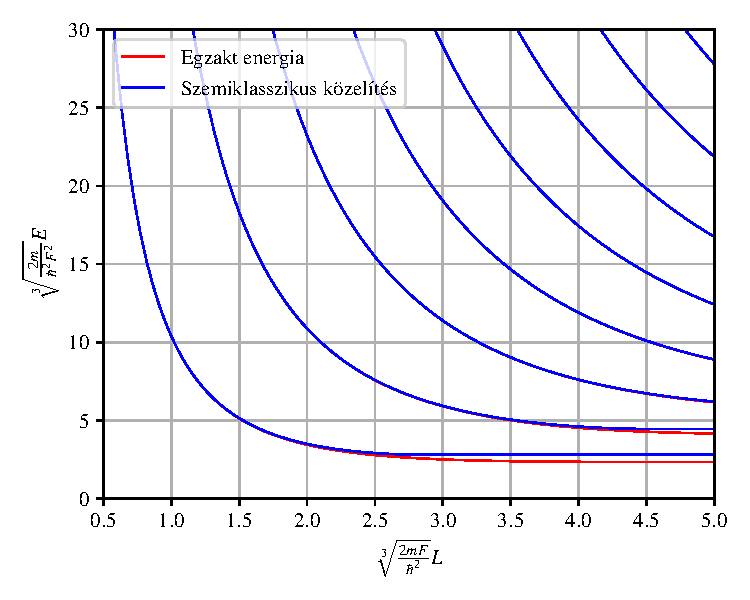
\includegraphics[scale=1]{./figs/energiaszintkozelites.pdf}
%		\caption[Szemiklasszikus energiaszintek]{Az ábra a szemiklasszikus energiaszinteket hasonlítja össze az egzakt energiaszintekkel. Ez az ábra is a $bE$ és $aL$ közötti relációt ábrázolja. A szemiklasszikus közelítés nagy kvantumszámok illetve $E \gg FL$ esetén pontos. Utóbbi oka, hogy ebben az esetben a potenciál elhanyagolható, és a potenciál nélküli végtelen potenciálgödör energiaszintjeit pedig a szemiklasszikus közelítés egzaktul megadja.}
%	\end{figure}
%	
%	\begin{figure}[H]
%		\centering
%		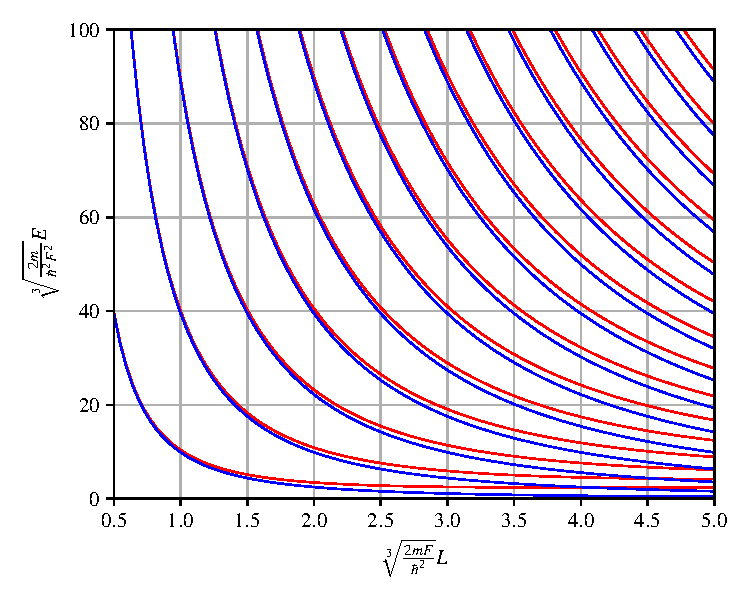
\includegraphics[scale=1]{./figs/infsquareenergia.pdf}
%		\caption[Végtelen potenciálgödör energiaszintjei]{Az ábrán a végtelen potenciálgödör és az egzakt energiaszintek összehasonlítása látható. Ez csak az $E \gg FL$ esetben jó közelítés, a szemiklasszikus energiaszintek jóval pontosabbak.}
%	\end{figure}
%
